% DOC SETTINGS ===================================
\documentclass{article}
\usepackage[utf8]{inputenc}
\usepackage{steinmetz}
\usepackage{mathtools}  
\usepackage{multicol}
\usepackage{circuitikz}
\usepackage{listings}
\usepackage{geometry}
\usepackage{fancyhdr}
\pagestyle{fancy}
\lhead{ECE2214 Lab Report 1}
\rhead{Kavin Thirukonda 2021}
\fancyheadoffset{0mm}
 \geometry{
 a4paper,
 total={170mm,257mm},
 left=20mm,
 top=25mm,
 }
\mathtoolsset{showonlyrefs} 
\cfoot{}
% DOC SETTINGS ===================================
\begin{document}
\begin{enumerate}
    \item 2 graphs comparing simulated and physical circuits.
        \begin{center}
            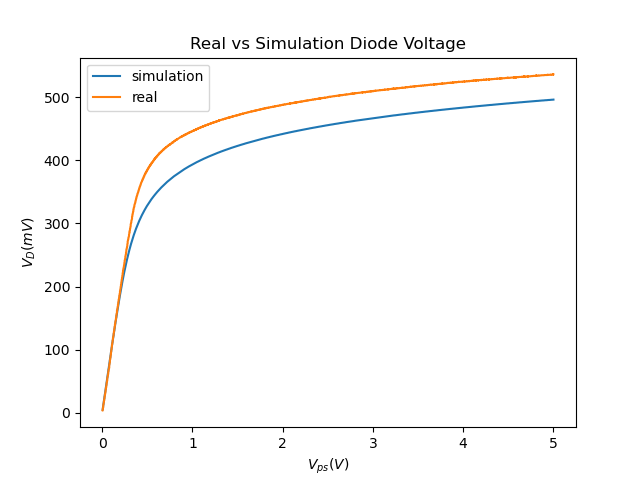
\includegraphics[width = .445\textwidth]{vd.png}
            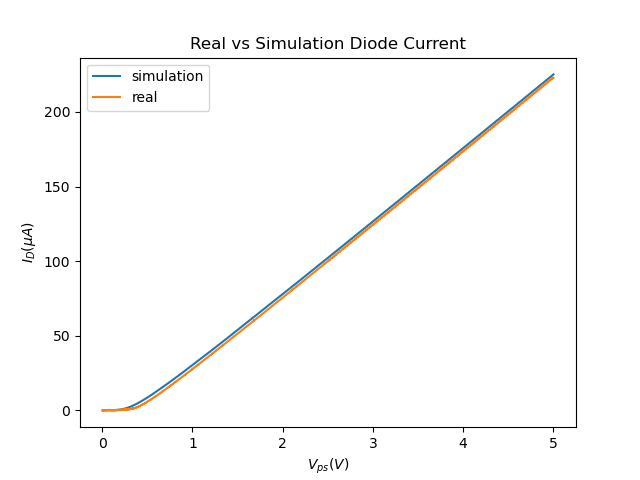
\includegraphics[width = .445\textwidth]{id.png}
        \end{center}
    \item Brief discussion of mismatch between the two circuits.
    \begin{center}
    The mismatch between the circuits could be due to a number of factors but the one I think is the most likely is the temperature difference between the simulation and the real. In the simulation I never specified a temperature but in real life the temperature is whatever it happens to be so it may be higher or lower than the simulation depending on the current room temperature.
    \end{center}
    \item Photo of physical circuit including Hokie Passport with Student ID number covered.
    \begin{center}
        \fbox{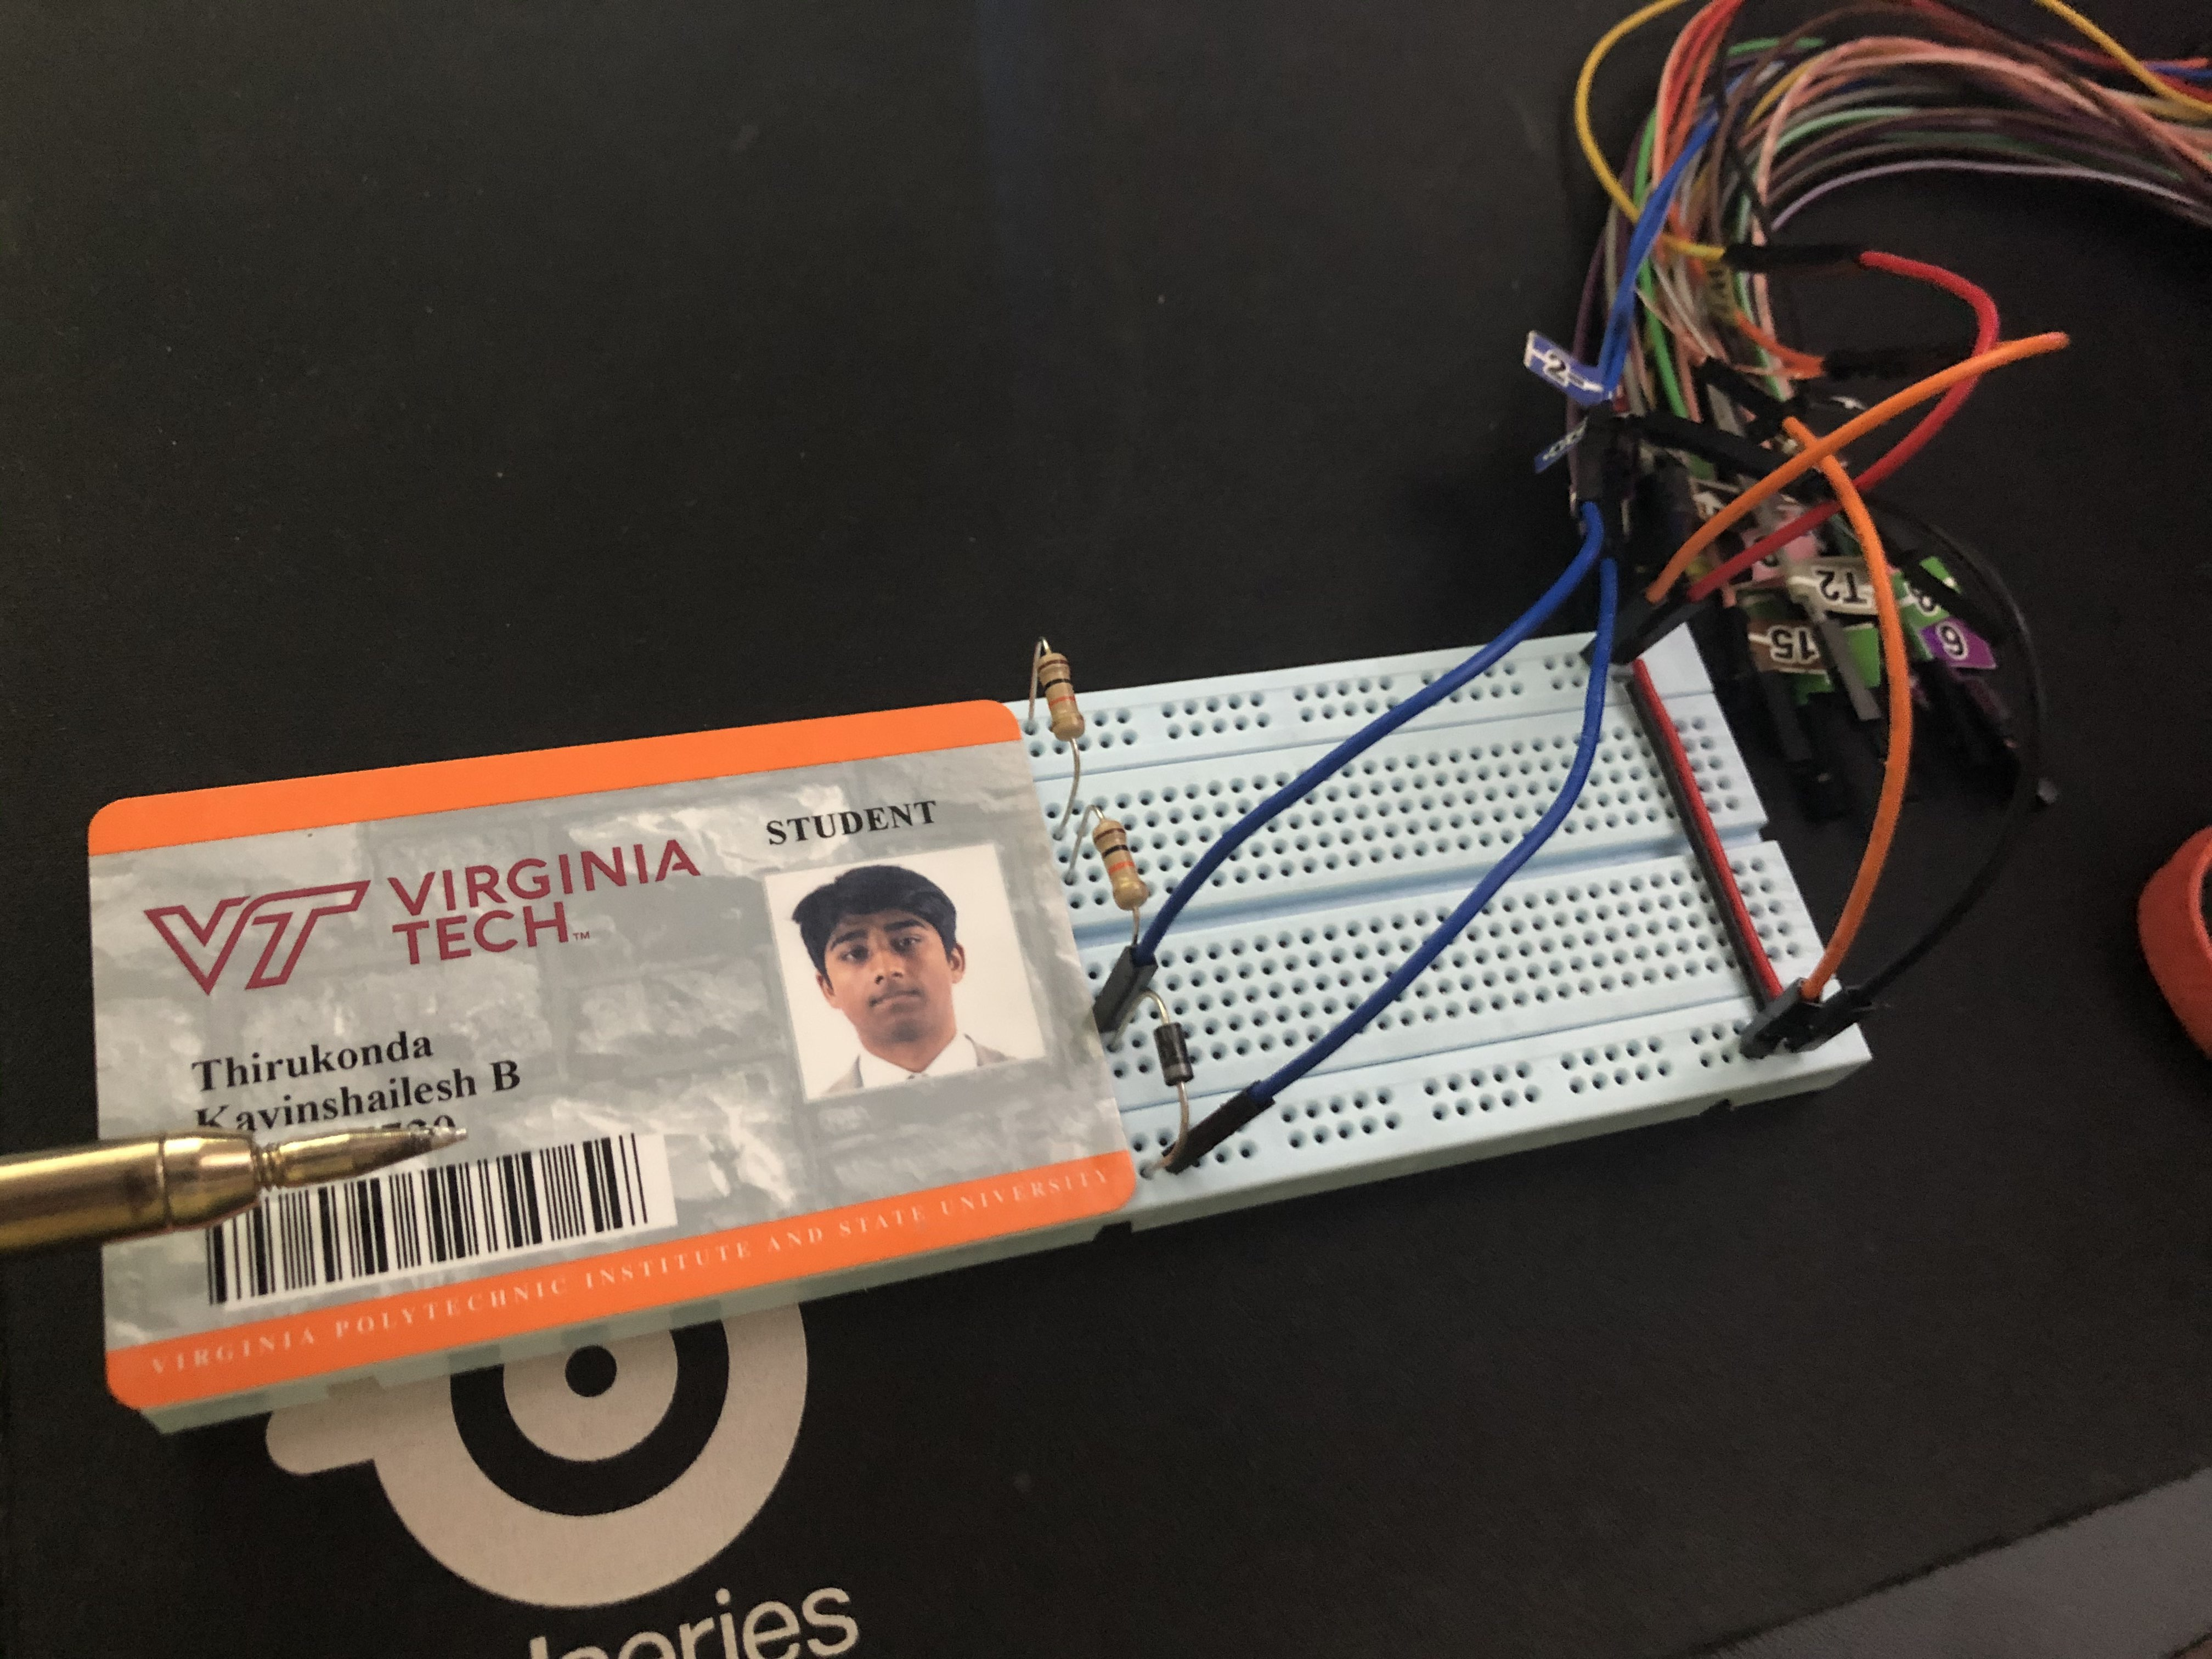
\includegraphics[width = .9\textwidth]{circuit.jpg}}
    \end{center}
    \newpage
    \item 2 graphs comparing simulated $I_D$ and $V_D$ for three separate temperatures.
    \begin{center}
        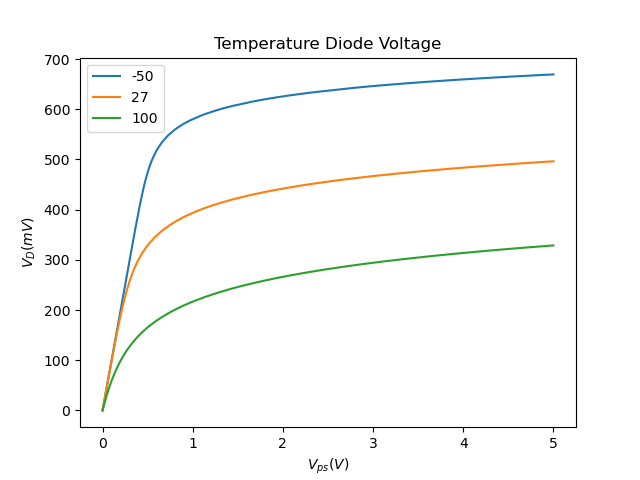
\includegraphics[width = .445\textwidth]{tempvd.png}
        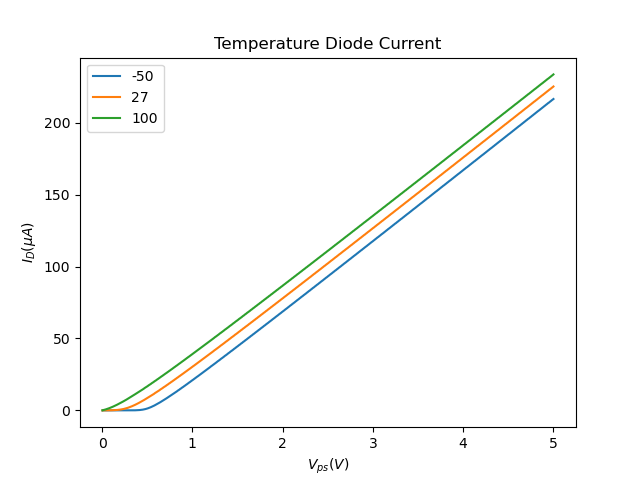
\includegraphics[width = .445\textwidth]{tempid.png}
    \end{center}
    \item Brief discussion of variation in results due to temperature sweep.
    \begin{center}
        because there is a lot of physics involved in semiconductors they are very dependent on factors like temperatures, and since diodes are just simple semiconductor junctions they too are very dependent on temperature and as can be seen with the graph above vary greatly across the range given to it.
    \end{center}
\end{enumerate}
\end{document}
